\documentclass[12pt,a4paper]{article}
\usepackage[utf8]{inputenc}
\usepackage[T1]{fontenc}
\usepackage{polski}
\usepackage[polish]{babel}
\usepackage{color}
\usepackage{cite}
\usepackage{url}
\usepackage{graphicx}


%element as landscape
\usepackage{pdflscape}
\usepackage{afterpage}

%listings
\usepackage{framed}
\usepackage{listings}
\usepackage[most]{tcolorbox}
\usepackage{filecontents}
\usepackage{tabularx}
\usepackage{caption}
%\tcbuselibrary{listings,breakable}

\lstdefinelanguage{JavaScript}{
  keywords={break, case, catch, continue, debugger, default, delete, do, else, false, finally, for, function, if, in, instanceof, new, null, return, switch, this, throw, true, try, typeof, var, void, while, with},
  morecomment=[l]{//},
  morecomment=[s]{/*}{*/},
  morestring=[b]',
  morestring=[b]",
  ndkeywords={class, export, boolean, throw, implements, import, this},
  keywordstyle=\color{blue}\bfseries,
  ndkeywordstyle=\color{darkgray}\bfseries,
  identifierstyle=\color{black},
  commentstyle=\color{purple}\ttfamily,
  stringstyle=\color{red}\ttfamily,
  sensitive=true
}
\newcounter{listing}
\setcounter{listing}{1}

\newtcbinputlisting{\jsfile}[3][]{%
  listing only,
  %titlepos=b,
  breakable,
  colframe=cyan,
  colback=white,
  left=6mm,
  title=Kod źródłowy \thelisting: #3,
  listing options={
    language=JavaScript,
    basicstyle=\small\ttfamily,
    breaklines=true,
    columns=fullflexible,
    numbers=left,numberstyle=\tiny\color{red!75!black},
    #1
  },
  listing file=#2
}

\newtcblisting{js}[1][]{
  listing only,
  breakable,
  colframe=cyan,
  colback=cyan!10,
  %title=#1,
  listing options={
    language=JavaScript,
    basicstyle=\small\ttfamily,
    breaklines=true,
    columns=fullflexible,
  },
  #1
}

\addto\captionspolish{\renewcommand*{\tablename}{Tabela}}


\begin{document}

\title{Zalecenia odnośnie pisania prac inżynierskich}
\author{Krzysztof Podlaski}
\date{}
\maketitle


\section{Uwagi ogólne}
\begin{itemize}
\item Wszystkie prace muszą spełniać wymagania opisane w regulaminie prac dyplomowych.
\item Część pisemna pracy inżynierskiej może być tworzona w dowolnej technologii (word, latex, openoffice, ...), proszę o przesyłanie do mnie wersji pdf. Osobiście polecam latex ale jest to tylko sugestia :-).
\item W trakcie pracy nad treścią pracy nie poprawiam tekstu, jedynie dodaję komentarze do dokumentu pdf.
\item Proszę o założenie na potrzeby projektu repozytorium git/bitbucket, abym miał dostęp do aktualnej wersji kodu programistycznego.  Repozytorium może być publiczne lub prywatne, w przypadku prywatnego proszę o dodanie mnie do tego repozytorium.
\item W trakcie pracy nad projektem inżynierskim proszę pamiętać o tym co nauczyliście się w trakcie przedmiotu inżynieria oprogramowania. Nie wymagam pracy w modelu kaskadowym (waterfall). Pewnie wygodniejsza jest jedna z metodyk iteracyjnych, zwinnych. Jednakże, każda z~nich wymaga aby każda z poniższych faz występowała co najmniej jednokrotnie:
    \begin{itemize}
    \item analizy wymagań,
    \item projektowania,
    \item implementacji,
    \item testowania.
    \end{itemize}
    W przypadku stosowania modelu iteracyjnego często fazy występują kilkukrotnie. Wymienione fazy muszą/powinny mieć swoje odzwierciedlenie w części pisemnej pracy inżynierskiej. Z mojego punktu widzenia bardzo ważne są dwie pierwsze oraz ostatnia z faz, one odzwierciedlają profesjonalizm dyplomanta. Jakość pracy wykonanej w trakcie implementacji świadczy o kompetencjach technologicznych.
\item Programistyczna praca inżynierska wymaga dobrej dokumentacji projektu (patrz Sekcja \ref{dokumentacja}).
\item Zalecam tworzenie bibliografii w miarę pisania pracy. Podejście ``dodam później'', niestety stosowane, zwykle wychodzi bokiem.
\item To samo dotyczy formatowania, w przypadku korzystania z word bądź openoffice zalecam od samego początku wykorzystywać odpowiednie style, aby można było później łatwo zmieniać format całego dokumentu. Zostawianie tego na sam koniec powoduje często problemy i ``rozjeżdżanie się'' pracy.
\end{itemize}

\section{Forma}

\subsection{Język}
Praca powinna być napisana poprawnie w języku polskim. Proszę zwrócić uwagę na wszelakie anglicyzmy często występujące w slangu informatycznym. W miarę możliwości stosujmy polskie słowa, jeżeli nie da rady łatwo zastąpić słowa angielskiego, należy tak przeformułować zdanie aby nie była wymagana odmiana słowa, a co za tym idzie konieczności dodawania polskiej końcówki do słowa angielskiego.
\begin{description}
  \item[{\color{red}Źle:}] Na potrzeby pracy usługi \underline{RESTowe} zostały stworzone z wykorzystaniem \underline{frameworka} Spring.
  \item[Poprawnie:] Na potrzeby pracy w celu stworzenia usług typu \underline{REST} wykorzystano \underline{framework} Spring.
\end{description}

Dodatkowo sugeruję stosowanie twardych spacji w celu unikania wszelkiego rodzaju sierotek, przed ostatecznym wysłaniem pracy do APD proszę o sprawdzenie czy nie występują  bękarty, sierotki, wdowy i szewcy \cite{Bekart}.

\subsection{Rozdziały}
Nie ma ogólnych założeń co do podziału logicznego pracy, przykładowy podział pracy na rozdziały poświęcone kolejnym zagadnieniom:
\begin{enumerate}
\item Wstęp - powinien zawierać ogólny opis celów pracy
\item Analiza wymagań,
\item Opis metod i technologii wykorzystanych w pracy,
\item Opis implementacji (dokumentacja projektu),
\item Testy aplikacji,
\item Instrukcja instalacji/obsługi,
\item Podsumowanie,
\item Bibliografia.
\end{enumerate}

\subsection{Odwołania}

\subsubsection{Bibliograficzne}
W pracy należy stosować jeden z trzech systemów cytowań (Vancouver System, Harvard System, Oxford System) opisanych szczegółowo w \cite{Cytowanie}, regulamin dyplomowania zaleca wykorzystanie systemu \underline{Vancouver}. W~przypadku systemów Vancouver i Oxford bibliografia powinna być posortowana w kolejności pojawiania się odwołań w tekście, natomiast w systemie Harvard alfabetycznie wedle nazwisk pierwszych autorów.

\subsubsection{Elementy pływające}
Każdy element pływający jak: obrazek, schemat, tabela czy fragment z~kodem źródłowym powinien zostać odpowiednio oznaczony (ponumerowany) i~zatytułowany. W~pracy powinno znaleźć się co najmniej jedno odwołanie do wspomnianego elementu, w~innym wypadku sprawia to wrażenie, iż element jest zbędny. Dodatkowo należy pamiętać, iż zasady umieszczania elementów pływających w~tekście ograniczają znacząco jaką część strony mogą zawierać, a~co za tym idzie omawiana tabelka, obrazek nie muszą znajdować się w~bezpośrednim sąsiedztwie tekstu odnoszącego się do obiektu.

\section{Dokumentacja Projektu}\label{dokumentacja}

\subsection{Wymagania aplikacji}
Praca powinna zawierać analizę wymagań aplikacji, każda forma stosowana w~inżynierii oprogramowania jest odpowiednia \cite{IO}, dodatkowo do opisu założeń aplikacji należało by wykorzystać przypadki użycia (Use Cases) \cite{UML}.

\begin{figure}[h]
\centering
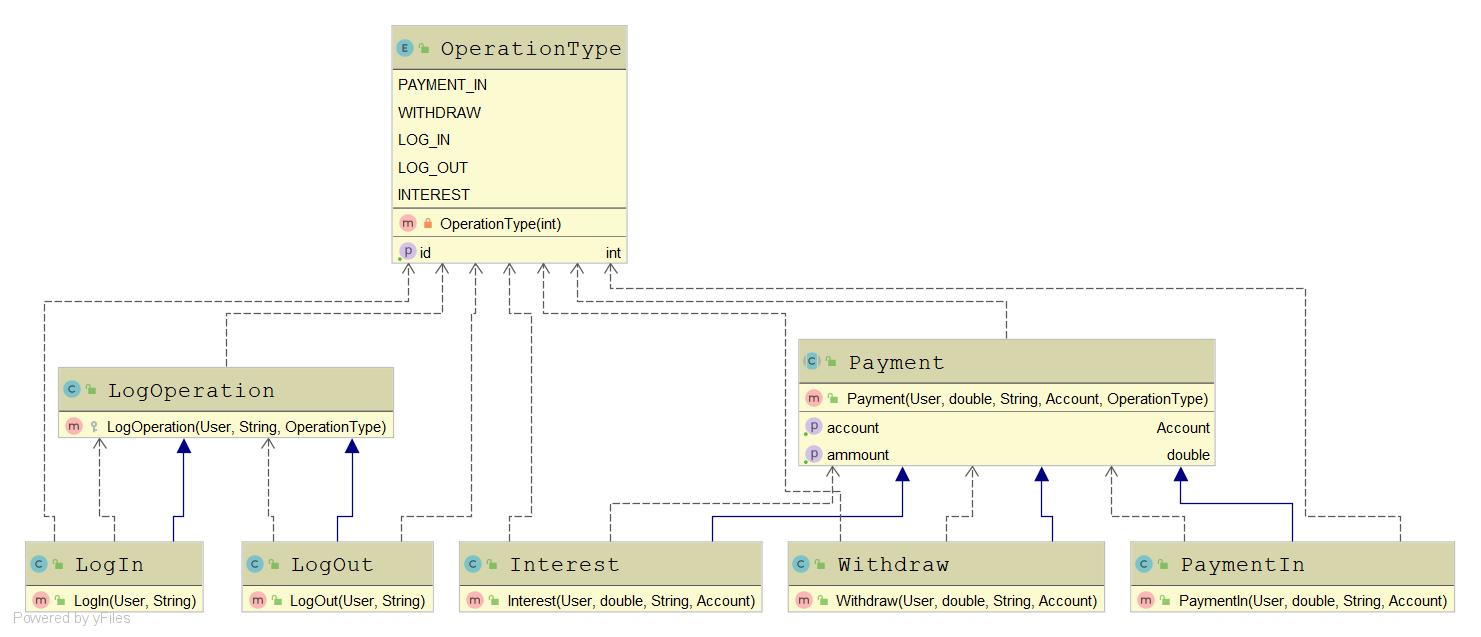
\includegraphics[width = \textwidth]{DiagramKlasPakiet.jpg}
\caption{Przykładowy diagram klas w wybranym pakiecie i zależności pomiędzy nimi.}\label{diagram_klas_pakiet}
\end{figure}


\subsection{Architektura aplikacji/systemu}
Bardzo często aplikacja/system tworzony w ramach pracy inżynierskiej składa się z wielu elementów jak np. baza danych, aplikacja serwerowa, aplikacja kliencka (mobilna). W pracy należy wyraźnie przedstawić podział na elementy składowe i metodę komunikacji pomiędzy nimi. Zalecanym sposobem przedstawienia zależności pomiędzy częściami projektu, oprócz opisu słownego, jest stosowanie schematów.

\subsection{Dokumentacja kodu}
 Poprawnym sposobem dokumentacji struktury klas jest diagram klas. Możemy stosować różnego rodzaju diagramy, bardzo ogólny reprezentujący strukturę całej aplikacji Rys.~\ref{duzy_diagram_klas}, jak i diagramy opisujące poszczególne pakiety Rys.~\ref{diagram_klas_pakiet} bądź pojedyncze klasy Rys.~\ref{diagram_wybranej_klasy}. Do diagramów klas należy dołączyć bardziej szczegółowy opis klasy, informujący użytkownika za co klasa odpowiada, jakie są jej pola, metody i ich parametry, w tym celu można wykorzystać postać tabelaryczną (Tab.~\ref{Opis_Klasy}) lub przedstawić opis w tekście pracy. W~przypadku prac zawierających znaczną ilość klas i ich metod nie wymagam aby wszystkie metody/pola zostały opisane w pracy. W~części  pisemnej należy opisać jedynie najistotniejsze metody/pola, dodatkowo należy stworzyć dokumentację techniczną klas za pomocą odpowiedniego narzędzia (doxygen, javadoc, ...) i~dodać do pracy w postaci załącznika w formie elektronicznej (na płycie CD/DVD).

\begin{figure}[!h]
\centering
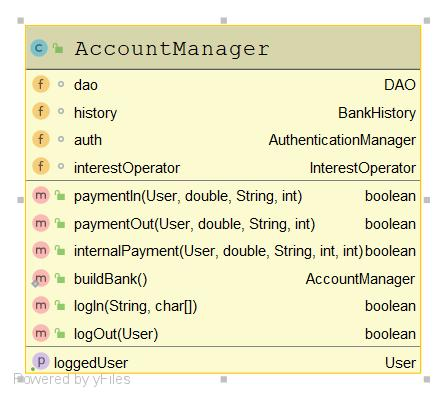
\includegraphics[width = 200pt]{DiagramKlasy.jpg}
\caption{Przykładowy diagram opisujący jedną klasę.}\label{diagram_wybranej_klasy}
\end{figure}

\begin{table}[!h]
\begin{center}
\begin{tabularx}{\textwidth}{|l|X|}
  \hline
  % after \\: \hline or \cline{col1-col2} \cline{col3-col4} ...
  Nazwa metody  & paymentOut  \\\hline
  Opis metody   & dokonanie przez użytkownika wpłaty na konto bankowe\\\hline\hline
  \multicolumn{2}{|c|}{parametry wejściowe} \\\hline
  user: User            &  reprezentuje użytkownika dokonującego wpłaty  \\\hline
  ammount: double       &  kwota do wpłacenia  \\\hline
  description : String  & opis wpłaty \\\hline
  accountId: int        & numer id konta na które należy dokonać wpłaty środków \\\hline\hline
  \multicolumn{2}{|c|}{parametry wyjściowe}   \\\hline
  typ boolean &  czy operacja zakończyła się sukcesem\\\hline\hline
  \multicolumn{2}{|c|}{Uwagi dodatkowe}\\\hline
  możliwe wyjątki   & \textit{OperationIsNotAllowedException} \\
                    & wyjątek tworzony w przypadku gdy użytkownik nie ma prawa wypłaty z podanego konta\\
                    & \textit{SQLException}\\
                    & wyjątek tworzony w przypadku kiedy nie ma  konta o zadanym accountid\\\hline
  podejmowane działania & W trakcie działania metody wszelkie operacje  podlegają logowaniu z wykorzystaniem pola history\\
  \hline
\end{tabularx}
\caption{Szczegółowy opis metody paymentOut klasy AccountManager.}\label{Opis_Klasy}
\end{center}
\end{table}



Działanie aplikacji, kodu aplikacji, powinno zostać zaprezentowane z wykorzystaniem diagramów UML\cite{UML}: sekwencji (Sequence diagram), aktywności (Activity diagram), stanu (State diagram) bądź schematów blokowych.  Jeżeli autor pracy uzna, że fragment kodu jest niezbędny, należy zastosować krótki jego fragment (do 10-20 linijek kodu). Proszę o unikanie wklejania do dokumentu fragmentów kodu źródłowego aplikacji. Dodatkowo nie zalecam używania w tym celu zrzutów ekranu z środowiska programistycznego, powoduje to często różne rozmiary czcionek w zależności od rozmiaru wyciętego fragmentu. Dodatkowo kod powinien być kolorowany na białym tle, nie należy stosować motywów typu kolorowy tekst na czarnym tle - wygląda to dużo gorzej na papierze i zużywa mnóstwo tonera, tuszu. Mile widziana jest numeracja linii co ułatwia późniejsze odnoszenie się do przedstawionego kodu źródłowego. Kolorystyka i obramowanie kodu nie musi przypominać tego umieszczonego w dokumencie (Kod~źr.~1), jednakże kod źródłowy musi się wyraźnie odróżniać od reszty tekstu pracy.

\jsfile[label=kod1]{code3.js}{Kod źródłowy obiektu app}



\subsection{Dokumentacja baz danych}
Praca musi zawierać informację o strukturze wykorzystywanych baz danych. W przypadku stosowania baz relacyjnych zaleca się postać diagramów opisujących tabele i relacje pomiędzy nimi, w natomiast przypadku baz obiektowych diagramy obiektów.

\afterpage{%
    \clearpage% Flush earlier floats (otherwise order might not be correct)
    \thispagestyle{empty}% empty page style (?)
    \begin{landscape}% Landscape page
        \begin{figure}
            \centering % Center table
            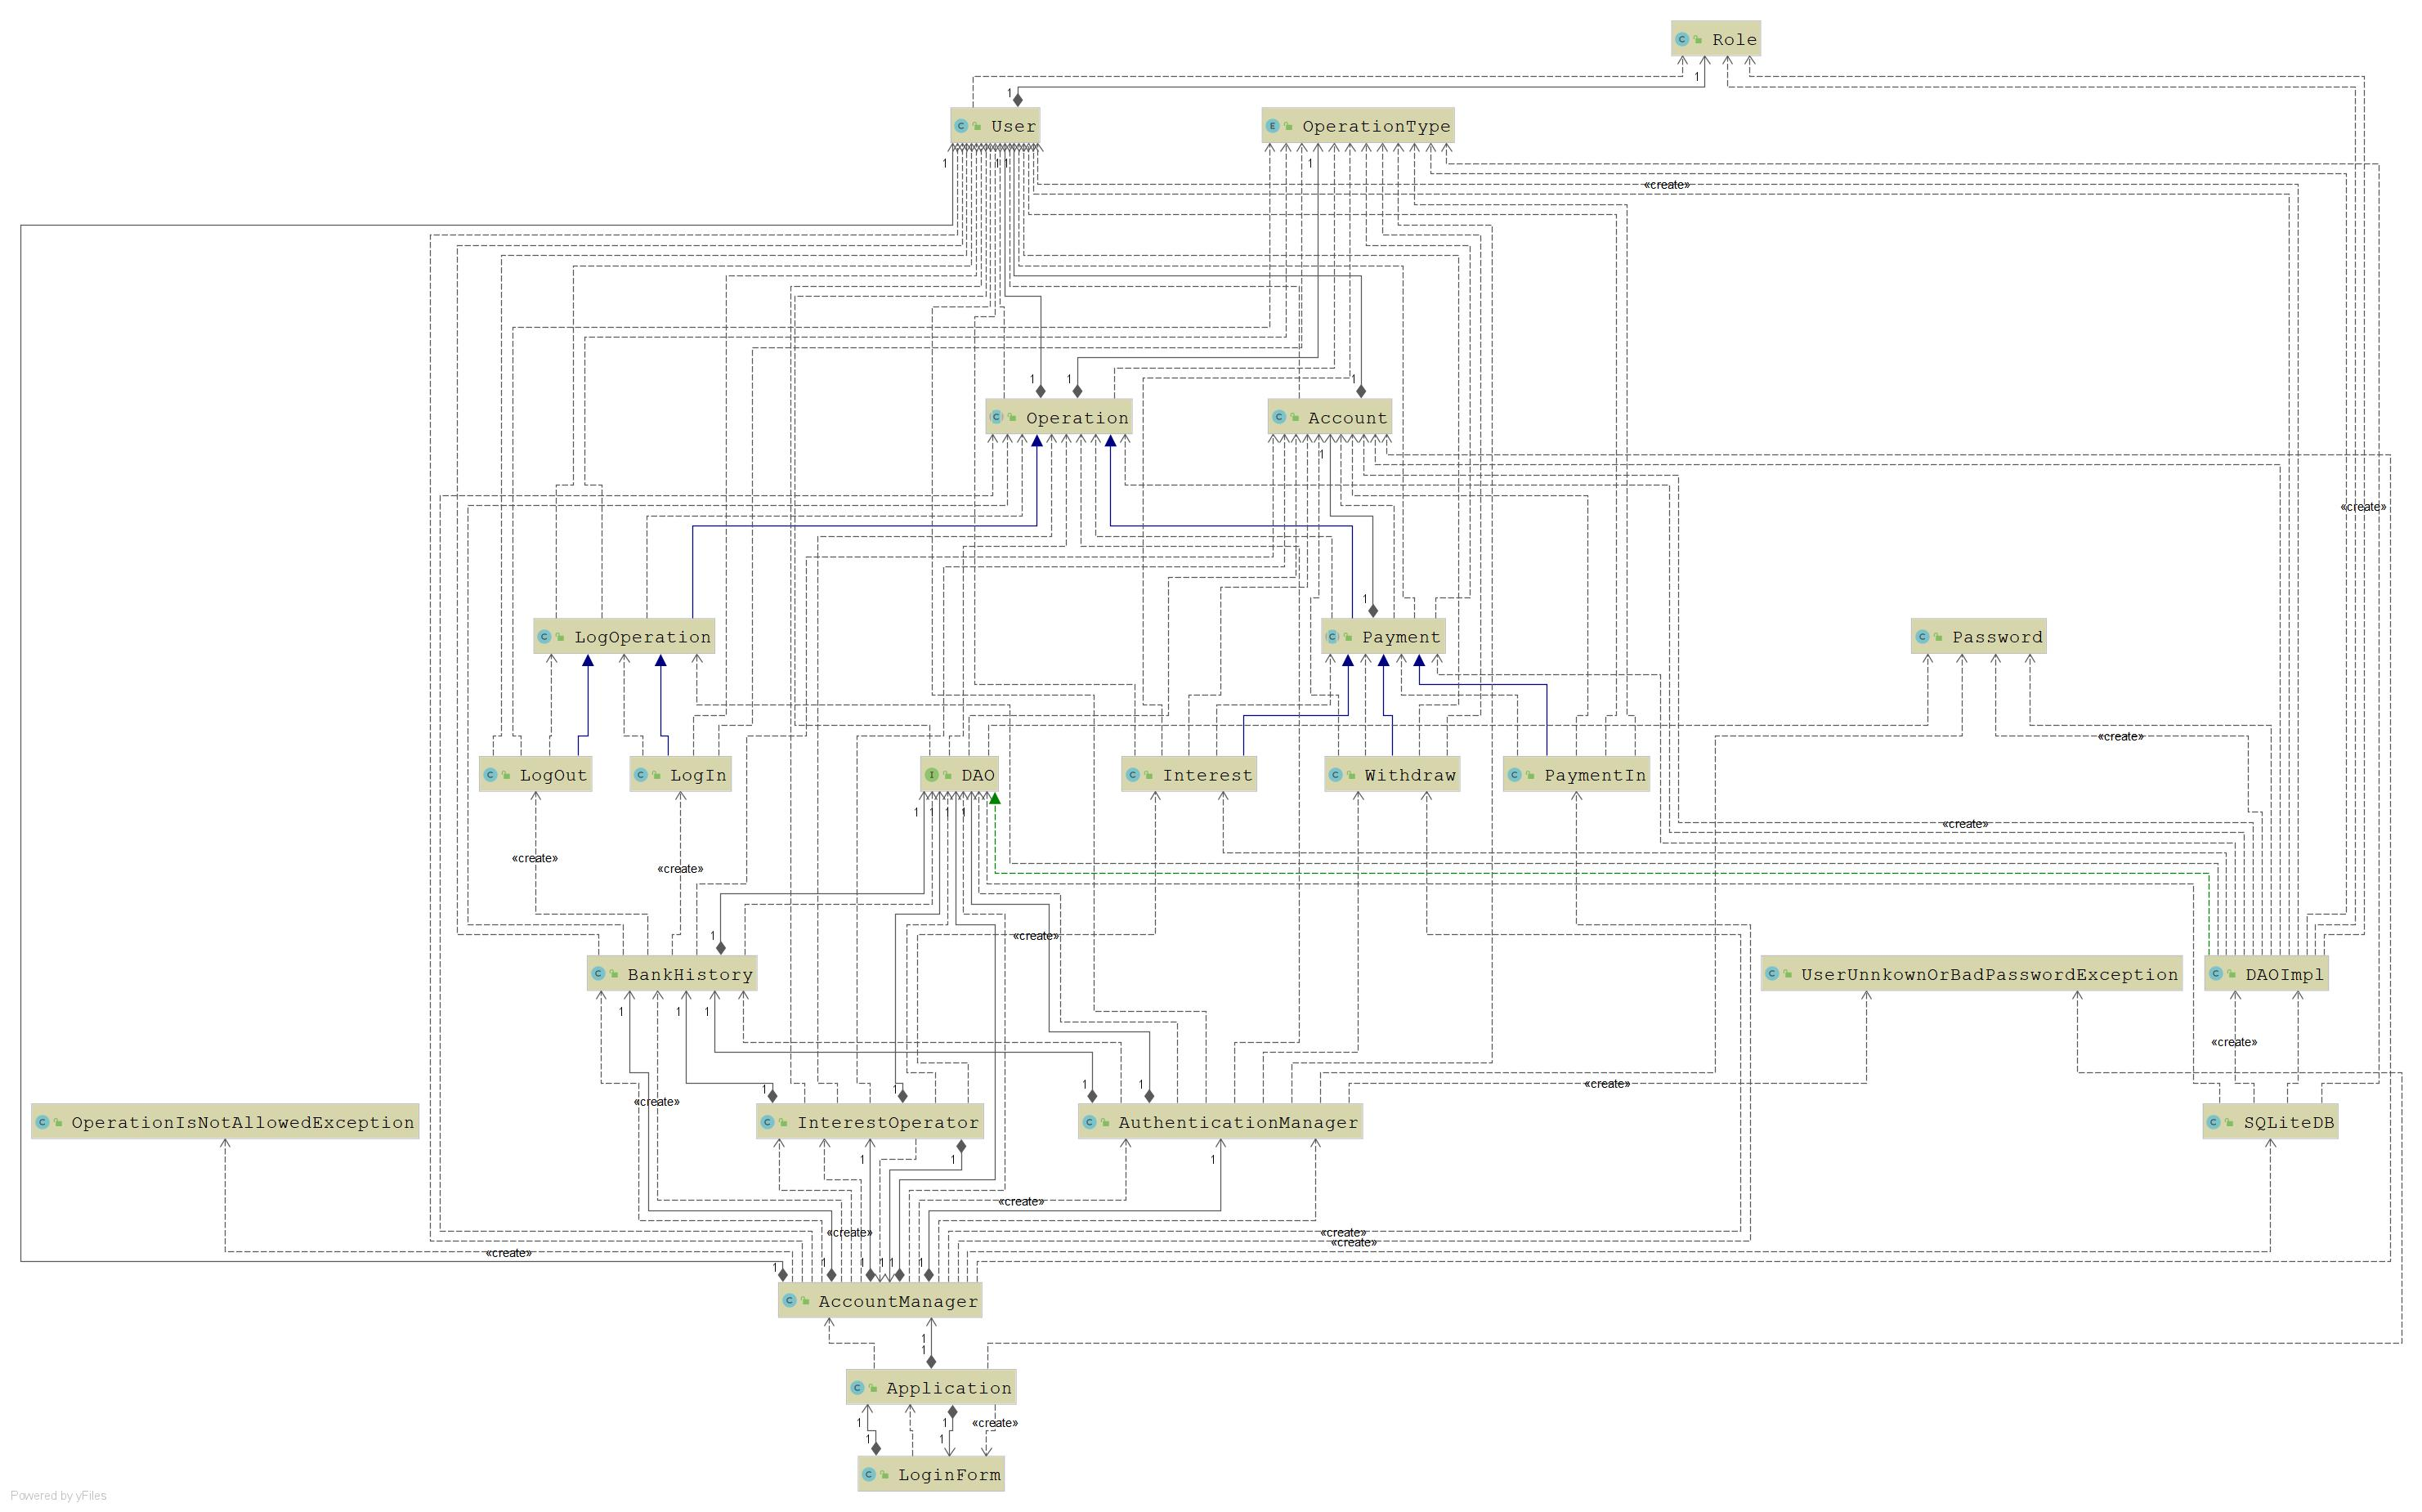
\includegraphics[width=1.5\textwidth]{DiagramKlasBig.jpg}
            \caption{Przykładowy ogólny diagram klas dla całej aplikacji.}\label{duzy_diagram_klas}
        \end{figure}
    \end{landscape}
    \clearpage% Flush page
}



\subsection{Protokoły wymiany informacji}
Jeżeli aplikacja zakłada wymianę danych pomiędzy elementami systemu, lub aplikacjami zewnętrznymi np z wykorzystaniem SOAP lub REST, należy opisać dokładnie protokół wymiany informacji, dla przykładu opis protokołu REST zawierają Tabele~\ref{rest1},~\ref{rest2}.

\begin{table}
\begin{tabularx}{\textwidth}{|l|X|}
\hline
&\textbf{Pobranie wybranego rekordu}\\\hline
URL &   \url{http://geniusgamedev.eu/cordova/rest_api/rest_srv/:id} lub \url{http://geniusgamedev.eu/cordova/rest_api/rest.php?id=:id}\\\hline
Method  & GET\\\hline
Parameters  & id - id wybranego elementu \\\hline
Request Data & None\\\hline
Response Data & obiekt w postaci:\\
&

%\begin{js}
\{'data':\{
    'id':2,
    'name':'Helena',
    'score':128
    \}
\}
%\end{js}

\\\hline
\end{tabularx}
\caption{Metoda get stosowanej usługi REST}\label{rest1}
\end{table}

\begin{table}
\begin{tabularx}{\textwidth}{|l|X|}
\hline
&\textbf{Dodanie nowego recordu}\\\hline
URL &   \url{http://geniusgamedev.eu/cordova/rest_api/rest_srv} or \url{http://geniusgamedev.eu/cordova/rest_api/rest.php}\\\hline
Method  & POST\\\hline
Parameters  & brak \\\hline
Request Data & nowy obiekt w postaci:\\
&\{
'data': \{
'id': 1,
'name': 'Jane',
'score': 332
\}
\}
\\\hline
Response Data & obiekt w postaci:\\
&
\{'data':\{
    'id':12,
    'name':'Jane',
    'score':332
    \}
\}
\\
&nowa wartość id została przypisana przez serwer w trakcie rejestracji obiektu.
\\\hline
\end{tabularx}
\caption{Metoda post stosowanej usługi REST}\label{rest2}
\end{table}



\subsection{Dokumentacja interfejsu użytkownika}
Dokumentacja interfejsu użytkownika powinna pokazywać przepływ pomiędzy widokami, na przykład za pomocą diagramu stanów (State diagram), dodatkowo możliwe jest wykorzystanie schematów typu UI-mockups reprezentujących rozłożenie elementów widoku. Obrazy przedstawiające rzeczywisty wygląd ekranów aplikacji (zrzuty ekranów) powinny raczej zostać umieszczone w instrukcji obsługi.


\subsection{Dokumentacja Testów}

Na potrzeby pracy należy wykonać testy manualne i/lub automatyczne. Mile widziane jest zastosowanie testów jednostkowych, interfejsu użytkownika czy akceptacyjnych. Testy należy opisać w postaci: wyszczególnionych przypadków testowych, każdy przypadek testowy powinien zawierać opis sposobu wykonania, kroków niezbędnych do jego przeprowadzenia.





\thebibliography{99}



\bibitem{Bekart} Strony Wikipedii poświęcone błędom w łamaniu tekstu\\
\url{https://pl.wikipedia.org/wiki/B%C4%99kart_(typografia)}

\bibitem{Cytowanie} Strona Wikipedii poświęcona metodom cytowania \\
\url{https://pl.wikipedia.org/wiki/Cytowanie_pi%C5%9Bmiennictwa}

\bibitem{IO} Ian Sommerville, Software Engineering, 10h ed., Pearsons  (2016)\\
 wydanie polskie Ian Sommerville, Inżynieria Oprogramowania, WNT (2003)

\bibitem{UML} Pascal Roques, UML in Practice: The Art of Modeling Software Systems Demonstrated through Worked Examples and Solutions, John Wiley \& Sons, 2004\\
    Przykładowy rozdział książki dotyczący wybranych diagramów UML i przypadków użycia \url{https://people.ok.ubc.ca/bowenhui/310/8-UML.pdf}

\end{document}
